\documentclass[a4paper,ngerman,oneside,titlepage,bibliography=totoc,11pt]{scrreprt}


\pagestyle{headings}

\usepackage{geometry}
\geometry{left=31mm, top=34mm, right=31mm, bottom=34mm}

\renewcommand{\ttdefault}{lmtt}
\linespread{1.06} %font

\usepackage[font=small,labelfont=bf]{caption} %caption, caption-font
\usepackage{subcaption}

\usepackage{amsmath, amsthm, amssymb, amsbsy}
\usepackage{mathtools}
\usepackage{color}
\usepackage{booktabs}
\usepackage{svg}

\usepackage[ngerman]{babel}
\usepackage[utf8]{inputenc} % für Umlaute (ansinew Editor, utf8 bei Texniccenter/Texmaker)
\usepackage[T1]{fontenc} % korrekte Trennung von Umlauten

\usepackage[hyphens]{url}
\usepackage{hyperref}
\usepackage{animate}
\usepackage{rotating}




\begin{document}


\begin{titlepage}

\newcommand{\HRule}{\rule{\linewidth}{0.5mm}} % Defines a new command for the horizontal lines, change thickness here

\center % Center everything on the page
 
%----------------------------------------------------------------------------------------
%	HEADING SECTIONS
%----------------------------------------------------------------------------------------

\LARGE Ludwig-Maximilians-Universität München\\[0.2cm] % Name of your university/college
\LARGE Institut für Statistik\\[5mm]% Major heading such as course name
\large Projekt im Rahmen des statistischen Consultings\\[6mm]
% Minor heading such as course title

%----------------------------------------------------------------------------------------
%	TITLE SECTION
%----------------------------------------------------------------------------------------

\HRule \\[0.4cm]
{ \huge \bfseries Internationaler Waffenhandel:\vspace{-1.5mm} Die Anwendung neuer Verfahren der\\[1mm] statistischen Netzwerkanalyse}\\[5mm]
{ Eine Netzwerkanalyse des internationalen Kleinwaffenhandels 1992 - 2011}\\
{ Kooperation mit dem Lehrstuhl für empirische Politikforschung}\\[0.4cm] % Title of your document
\HRule \\[1.5cm]
 
%----------------------------------------------------------------------------------------
%	AUTHOR SECTION
%----------------------------------------------------------------------------------------

\begin{minipage}[t]{0.4\textwidth}
\begin{flushleft} \large
\emph{Autor:}\\[2mm]
Felix Loewe\\
loewe.felix@gmail.com\\[5mm]


\end{flushleft}
\end{minipage}
~
\begin{minipage}[t]{0.4\textwidth}
\begin{flushright} \large
\emph{Projektpartner:}\\[2mm]
Prof. Dr. Paul W. Thurner\\[6mm]

\emph{Betreuer:}\\[2mm]
Prof. Dr. Göran Kauermann\\[6mm]
\end{flushright}
\end{minipage}\\[4.5cm]

\end{titlepage}




\begin{abstract}


\begin{center}
{\it \bf Abstract} 
\end{center}
Dieser Bericht behandelt die Analyse der \emph{NISAT database of transfers of small arms, light weapons, and their ammunition, parts and accessories}. Die Netzwerkdaten stellen das internationale Kleinwaffenhandelsnetzwerk im Zeitraum 1992 bis 2011 dar.

Nachdem die Datengrundlage besprochen wird, erfolgt eine deskriptive Analyse des Handelsnetzwerkes anhand Zeitreihen von Netzwerkstatistiken. Im zweiten Teil wird der Querschnitt des Netzwerkes Jahr für Jahr anhand von ERGMs modelliert, um charakteristische Strukturen des Netzwerkes aufzudecken. Der Fokus liegt hierbei auf der Selektion interner Netzwerkstatistiken sowie externer Kovariablen.
 \\
 
 {\bf Schlagwörter}\quad {\it Netzwerkanalyse -- Waffenhandel -- Kleinwaffen -- ERGMs}

\end{abstract}




\tableofcontents




\chapter{Einführung}

Was ist das Besondere an der statistischen Analyse von Netzwerken? Erstens stellen sie durch ihre Abhängigkeitsstruktur relationale Daten dar. Gewöhnliche Datensätze mit $i = 1, ..., N$ Beobachtungen werden zumeist mit der Annahme analysiert, dass die $n$ Beobachtungen unabhängig voneinander beobachtet werden. Bei Netzwerkdaten ist das nicht der Fall. Hier stehen die Beobachtungen, oft genannt \emph{Akteure} des Netzwerkes, in Beziehung zu einander. Besteht eine Beziehung zwischen den Beobachtungen, können diese nicht mehr als unabhängig angesehen werden. In ähnlicher Sichtweise wird auch eine nicht-bestehende Beziehungen nicht ignoriert, sondern so angesehen, dass individuenspezifische oder netzwerkspezifische Effekte diese verursacht haben können.

Das Bestehen- oder Nicht-Bestehen einer Beziehung ist die Netzwerkstruktur (\emph{Abhähngigkeitsstruktur}), die zusätzlich zu den Daten eines gewöhnlichen Datensatzes besteht. Die Abhängigkeitsstruktur wird durch die Adjazenzmatrix $Y_{ij} \in N \times N$ ausgedrückt.

Zweitens stellen Netzwerkdaten eine Verallgemeinerung von räumlichen Daten dar. Bei räumlichen Daten wird von der Nachbarschaftsstruktur gesprochen. Markov-Zufallsfelder können als Graph visualisiert werden, dessen Akteure räumliche Punkte oder zum Beispiel Länder sind.
Sind diese benachbart, besteht eine Kante. Zwei Punkte $i, j$ sind benachbart ($i \sim j$), falls der entsprechende Eintrag in der Adjazenzmatrix eine Eins aufweist. Netzwerke verallgemeinern das Konzept des räumlichen Nachbarns auf beliebige Beziehungen. Bei der Analyse des Waffenhandels wird aus der Beziehung ein Handel und aus den Akteuren die liefernden und belieferten Länder.

Die Arbeit ist wie folgt aufgebaut. Im ersten Kapitel erfolgt eine kurze Wiederholung der Begriffe aus der Graphentheorie. Diese Begriffe werden in den darauffolgenden Kapiteln verwendet, um weitere netzwerkstatistische Begriffe einführen zu können. Im zweiten Kapitel erfolgt eine Erläuterung der Datengrundlage der NISAT Datenbank. Im dritten Abschnitt wird der Datensatz deskriptiv analysiert. Im vierten Abschnitt erfolg die Modellierung per ERGMs.





\section{Wiederholung der Graphentheorie}

Um Netzwerkdaten statistisch analysieren zu können, muss die Abhängigkeitsstruktur der Daten adäquat modelliert werden. Eine grundlegende mathematische Theorie, die verwendet wird, um \emph{relationale Daten} zu beschreiben, ist die Graphentheorie. Die Notation der graphentheoretischen Begriffe orientiert sich an \cite{kc14}.

\subsection{Graph}

Ein Graph $G = (V,E)$ ist die mathematische Beschreibung eines Netzwerkes. 

Er besteht aus einer Knotenmenge $V$ und einer Kantenmenge $E$. Ein Knoten $v$ ist ein Punkt eines Graphen. Eine Kante $e$ verbindet zwei Punkte. Mit diesen zwei Begriffen kann ein Graph graphisch dargestellt werden.

Es wird eine Konvention getroffen, dass es nur eine endliche Zahl an Knoten in einem Graph gibt. Die Anzahl der Knoten wird mit $N_V = |V|$ bezeichnet. Üblicherweise sind die Knoten $v_i$ durchnummeriert mit dem Index $i = 1, ..., N_V$. 

Eine Kante $e$ ist ein Element der Menge $E$. Eine Kante $e = \{i,j\}$ beschreibt die Verbindung zwischen Knoten $v_i$ und $v_j$. 

Es gibt ungerichtete und ungerichtete Graphen. Sie unterscheiden sich darin, ob eine Kante, also die Beziehung zwischen den Akteuren, gerichtet oder ungerichtet ist. Ein Beispiel für ungerichtete Beziehungen ist eine Freundschaftsbeziehung. Ein Beispiel für eine gerichtete Beziehung ist der Kleinwaffenhandel: es gibt ein Export- und ein Importland. Das Kleinwaffenhandelsnetzwerk kann also durch einen gerichteten Graphen beschrieben werden.

Mathematisch unterscheiden sich gerichtete und ungerichtete Graphen darin, ob eine Kante $e$ ein geordnetes Paar $(i,j)$ oder ein ungeordnetes Paar $\{i,j\}$ ist. Die Kantenmenge $E$ eines gerichteten Graphs kann als Teilmenge des kartesischen Produkts $V \times V$ dargestellt werden.

Erweiterungen von Graphen stellen Graphen mit Schleifen und Multigraphen dar. Eine Schleife ist eine Kante der Form $(i,i)$. Multigraphen sind Graphen, die mehrere Kanten von einem Knoten zu einem anderen Knoten erlauben. Eine Multikante kann als Tupel $(e, r)$ definiert werden, wobei $e$ die gerichtete oder ungerichtete Kante bezeichnet, und $r$ die Anzahl der Multikanten. Um Graphen von Multigraphen zu unterscheiden, spricht man bei einem Graph ohne Multikanten von einem einfachen Graphen.

Betrachtet man die Anzahl der möglichen Kanten eines Graphen, die später als Benchmark dafür auftaucht, wie dicht ein Graph sein kann, so wird ersichtlich, dass diese Anzahl für einen einfachen ungerichteten Graphen kleiner ist als die Anzahl der möglichen Kanten einer komplizierteren Graphenart. Für einen einfachen ungerichteten Graphen ist sie gegeben durch:

$$V_H(V_H-1)/2$$

Werden Schleifen $\{i,i\}$ erlaubt, sind mehr Kanten möglich. Dann wird der Zähler durch $V_H^2$ ersetzt. Werden gerichtete Kanten $(i,j)$ erlaubt, kommen erneut mehr mögliche Kanten hinzu. Der Zähler wird dann nicht mehr durch Zwei geteilt.


\subsection{Adjazenzmatrix}

+Ein Graph ist vollständig bestimmt durch seine Adjazenzmatrix $A_{ij} \in |V| \times |V|$, wobei $a_{ij} = 1$ bedeutet, dass zwischen Knoten $i$ und Knoten $j$ eine Kante besteht.

+Bei gerichteten Graphen besteht ein Unterschied zwischen der Kante $(i,j)$ und der Kante $(j,i)$. Die Adjazenzmatrix ist dann nicht symmetrisch.


\section{Datengrundlage}



Die Datengrundlage für das Kleinwaffenhandelsnetzwerk ist die \emph{NISAT} (Norwegian Initiative on Small Arms Transfers) Datenbank. Das Peace Research Institute Oslo (PRIO) ist der Auftraggeber dieser Datenbank. Die Datenbank enthält Daten über den legalen und illegalen Handel von Kleinwaffen. Der abgedeckte Zeitraum beträgt die Jahre 1992 bis 2011. Berichtet wird hierin von insgesamt 239 Ländern und 109522 Waffentransaktionen.

Es folgt eine genauere Beschreibung der Datenbank. Die Daten liegen in Form von einer gerichteten Kanten-Liste vor. Das bedeutet jede zeile im Datensatz entspricht einem Handel zwischen einen exportierdenen und einem importierenden Land. Zusätzliche Attribute sind die Correlates of War Codes der jeweiligen Länder, der Monetäre Wert des Handels in US Dollar, der Waffentyp der gehandelt wurde, die Datenquelle die den Handel berichtet sowie das Jahr in dem der Handel stattgefunden hat.
Bei der Netzwerkanalyse dieser Daten erkennt man schnell folgende Probleme:
Da nach Waffentypen unterschieden wird, existieren in den einzelnen Jahren multiple Kanten. Das bedeutet zwischen 2 Ländern werden im gleichen Jahr mehrere Handel in der gleichen Richtung aufgeführt. Diese wurden für die weitere Analyse zusammengefasst indem der Wert der Lieferungen schlicht addiert wurde.
Der Datensatz enthält Schleifen. Das heißt manche Länder liefern Waffen an sich selbst. Da es hierfür keine sinnvolle inhaltliche Erklärung gibt wurden die entsprechenden Beobachtungen gelöscht.

\chapter{Deskriptive Analyse}

\section{Degree Sequenz}

\begin{figure}[h]
	\centering
		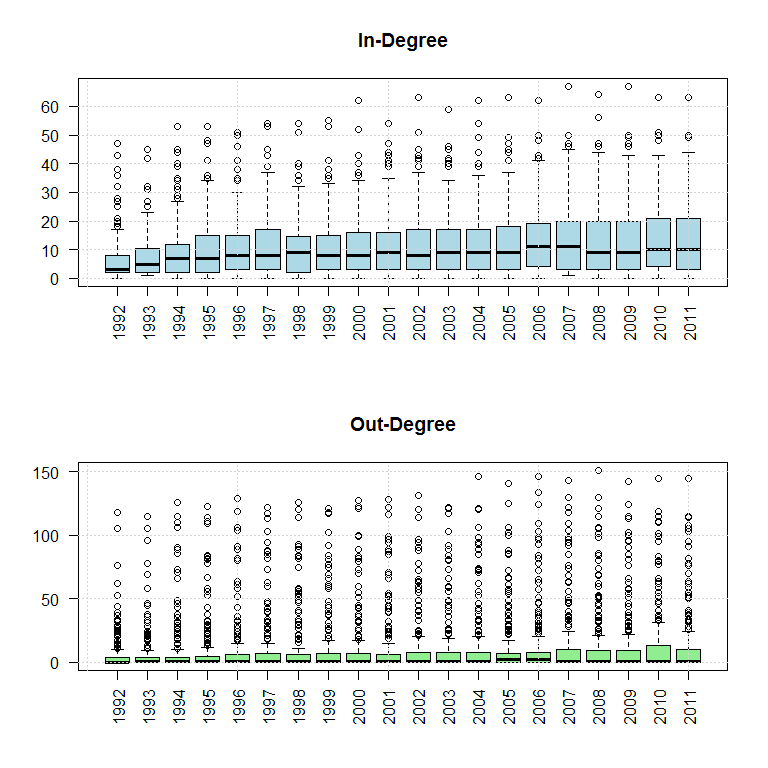
\includegraphics[width=1.00\textwidth]{Grafiken/ts_degree.png}
	\caption{Boxplot für In- und Out-Degree in den Jahren 1992-2011}
	\label{fig:ts_degree}
\end{figure}

Eine erste nützliche Analyse um die Struktur des Netzwerkes zu erfassen, ist die Betrachtung der Knoten-Degrees. Im Falle eines gerichteten Netzwerkes unterschiedet man zwischen In-Degree und Out-Degree. Inhaltlich interpretiert entspricht dies den Anzahlen der Importe und Exporte der Länder pro Jahr. Hierzu betrachten wir Abbildung \ref{fig.ts_degree}. Sie zeigt zu jedem im Datensatz enthaltenen Jahr je einen Boxplot zum In-Degree und einem zum Out-Degree. innerhalb der farblich gekennzeichneten Box liegen jeweils die mittleren 50 Prozent der entsprechenden Daten. Der mittlere Schwarze Strich in jeder box kennzeichnet den Median, und damit den Wert, unter dem genau die Hälfte aller Werte liegt.

Betrachtet man zuerst die Boxplots zum In-Degree, so stellt man fest, dass die breite der box über die Jahre zunimmt. Im Jahr 1992 reicht sie lediglcih von 2 bis 8, während sie sich im Jahr 2011 von 3 bis 21 erstreckt. Auch der Median steigt über diesen Zeitraum von  3 auf 10. Daraus lässt sich schließen, dass die mittlere ANzahl der Länder aus denen ein einzelnes Land Waffen exportiert größer geworden ist. Auffalend sind in allein Jahren einige mit Kreisen markierte Ausreißer
die aus bis zu 67 verschiedenen Ländern im gleichen Jahr waffen beziehen.

Bei den boxplots zum Out-Degree fallen sofort die sher kleinen Boxen auf. Übereinstimmend in allen Jahren exportieren mindestens 25 Prozent der Länder überhaupt keine Waffen, und 50 Prozent der Länder an höchstens 2 andere Staaten. Allerdings gibt auch in allen Jahren eine recht große Anzahl von Ausreißern mit hohem Out-Degree mit bis zu 150 belieferten Staaten. 

Die Betrachtung der Degrees legt nahe, dass der Kleinwaffenhandel von einigen wenigen Akteuren dominiert wird, während die große Masse der restlichen Staaten eher einen geringen Einfluss auf die Geschehnisse hat. Diesen wichtigen Akteuren wenden wir uns in Abschnitt \ref{sec:top-akteure} zu.

\section{Handelswerte}

\begin{figure}[h]
	\centering
		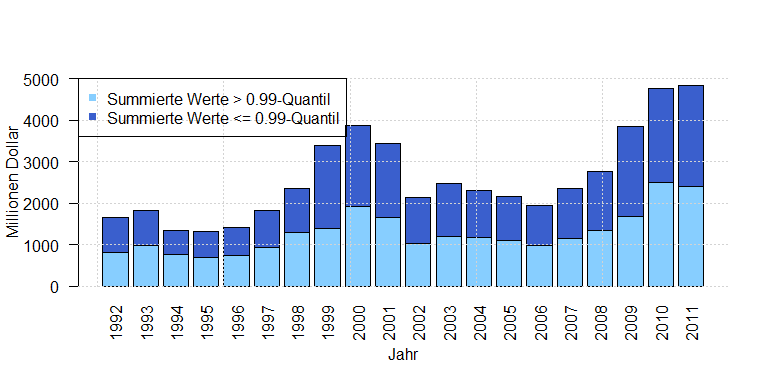
\includegraphics[width=1.00\textwidth]{Grafiken/ts_value.png}
	\caption{Vergleich der 1\% teuersten Waffenkäufe mit den 99\% billigsten}
	\label{fig:ts_value}
\end{figure}

Betrachtet man sich die gewichte der Kanten, in diesem Fall die monetären Handelswerte so fällt einen ein deutliches Ungleichgewicht auf. Wie Abbildung \ref{fig:ts_value} zeigt ist die Summe der 1\% teuersten Waffenhandel über alle Jahre hinweg ähnlich der Summe der 99\% billligsten. Einige wenige große Waffentransaktionen wiegen also alle restlichen in ihrem monetären und damit wohl auch quantitativen Gewicht auf.

\section{Top-Akteure}
\label{sec:top-akteure}
Als erstes wird darauf eingegangen, welches die zentralen Akteure des Handelsnetzwerkes sind. Das bedeutet, es werden die Nationen aufgelistet, die über den Zeitraum von 20 Jahren das größte Import- und Exportvolumen, gemessen am Geldwert der gehandelten Waffen, aufweisen. Die Top-Exporteure sind in Tabelle \ref{top_exp} zu sehen.

\begin{table}[h]
\centering
\footnotesize
\begin{tabular}{rlr}
  \hline
 Platz & Land & Exportvolumen [Mrd.]\\ 
  \hline
1 & United States of America & 9.2\\ 
  2 & Italy & 7.9 \\ 
  3 & Germany (Federal Republic) & 4.6 \\ 
  4 & Brazil & 3.7 \\ 
  5 & Austria & 2.7 \\ 
  6 & United Kingdom & 2 \\ 
  7 & Belgium & 1.8 \\ 
  8 & Switzerland & 1.5 \\ 
  9 & Russia / USSR (Former) & 1.4 \\ 
  10 & Czech Republic & 1.4 \\ 
   \hline
\end{tabular}
\caption{Top-Exporteure des Netzwerks} 
\label{top_exp}
	\end{table}
	
Es ist ersichtlich, dass die Vereinigten Staaten von Amerika mit 9.2 Milliarden Dollar am meisten Waffen exportiert. Italien steht mit circa 8 Milliarden Dollar Exportvolumen an zweiter Stelle. Dies erscheint ungewöhnlich über den Zeitraum von 1992 -- 2011. Deutschland exportiert mit circa 5 Milliarden Dollar gehandelten Waffen am drittmeisten. Auf dem vierten und fünften Platz folgen die Länder Brasilien und Österreich mit exportierten Waffen, die circa 4 und 3 Milliarden Dollar wert sind. Ab dem sechsten Platz erfolgen nur noch unwesentliche Verringerungen des Exportvolumens im Bereich von 2 bis 1 Milliarde Dollar. Hierin befinden sich Nationen wie Großbritannien, Belgien, die Schweiz, Russland und die tschechische Republik. 

Nun folgt eine Auflistung der Top-Importeure des Kleinwaffenhandelsnetzwerkes (siehe Tabelle \ref{top_imp}).

\begin{table}[h]
\centering
\footnotesize
\begin{tabular}{rlr}
  \hline
 Platz & Land & Importvolumen [Mrd.]\\ 
  \hline
1 & United States of America & 16\\ 
  2 & Germany (Federal Republic) & 2.3\\ 
  2 & France & 2.3\\ 
  4 & Canada & 1.9 \\ 
  5 & United Kingdom & 1.8\\ 
  6 & Saudi Arabia & 1.7\\ 
  7 & Belgium & 1.2\\ 
  8 & Spain & 1.2\\ 
  9 & Australia & 1.2\\ 
  10 & Turkey & 1\\ 
   \hline
\end{tabular}
\caption{Top-Importeure des Netzwerks} 
\label{top_imp}
	\end{table}
		
Erneut steht Nord-Amerika an erster Stelle. Die Nation gibt circa 16 Milliarden Dolar für den Import von Kleinwaffen aus. Deutschland und Frankreich teilen sich mit 2.3 Milliarden Dollar Importvolumen den zweiten Platz am Kleinwaffenimport. Auf der vierten Stelle befindet sich Kanda mit einem Importvolumen von circa 2 Milliarden Dollar. Großbritannien verwendet 1.8 Milliarden Dollar, um Waffen zu exportieren, und Saudi Arabien 1.7 Milliarden Dollar. Auf dem siebten, achten, neunten und zehnten Platz sehen wir ähnliche Exportausgaben von circa 1.2 bis 1 Milliarde Dollar. Dies sind die Länder Belgien, Spanien, Australien und Türkei.

Anschließend interesiert, ob sich die Zusammensetzung der Top-Exporteure/Importeure über die Jahre verändert. Hierfür betrachten wir Abbildung \ref{fig:ts_tops}. 
In der ersten Grafik sind die Handelsvolumen in Millionen US Dollar der fünf Top-Exporteure über den Zeitraum 1992-2011 dargestellt. Die USA ist in fast allen Jahren der Waffenexporteur mit den höchsten monetären Volumen. Sie wird nur in wenigen Jahren von Italien übertroffen. Deutschland, Brasilien und Österreich exportieren in allen Jahren deutlich weniger Waffenwert als die USA. Aufällig ist ein relativ konstanter Verlauf der Zeitreihen im Zeitraum von 1992 bis ca 2001, während danach bei allen Ländern ein kräftiger Anstieg der Handelswerte feststellbar ist. Deutschland, Brasilien und vor allem Italien zeigen allerdings ab ca 2008 widerum einen abfallenden Trend.
Die zweite und die dritte Grafik aus Abbildung \ref{fig:ts_tops} zeigt die Handelsvolumen der Top-Importeure. Die USA ist hier unangefochten an der Spitze. Sie importiert Kleinwaffen im Wert zwischen circa 400 und 1600 Millionen US Dollar pro Jahr während die restlichen Akteure höchstens Kleinwaffen im Wert von circa 250 Millionen Dollar pro Jahr importieren. Ähnlich wie bei den Exportzeitreihen ist auch hier ein relativ konstanter Verlauf bis ca 2001 zu beobachten während die Ausgaben in den nachfolgenden Jahren kontinuierlich ansteigen. Die USA verringerte ihre Importausgaben ab dem Jahr 2007 jedoch wieder deutlich. 

\begin{figure}[h]
	\centering
		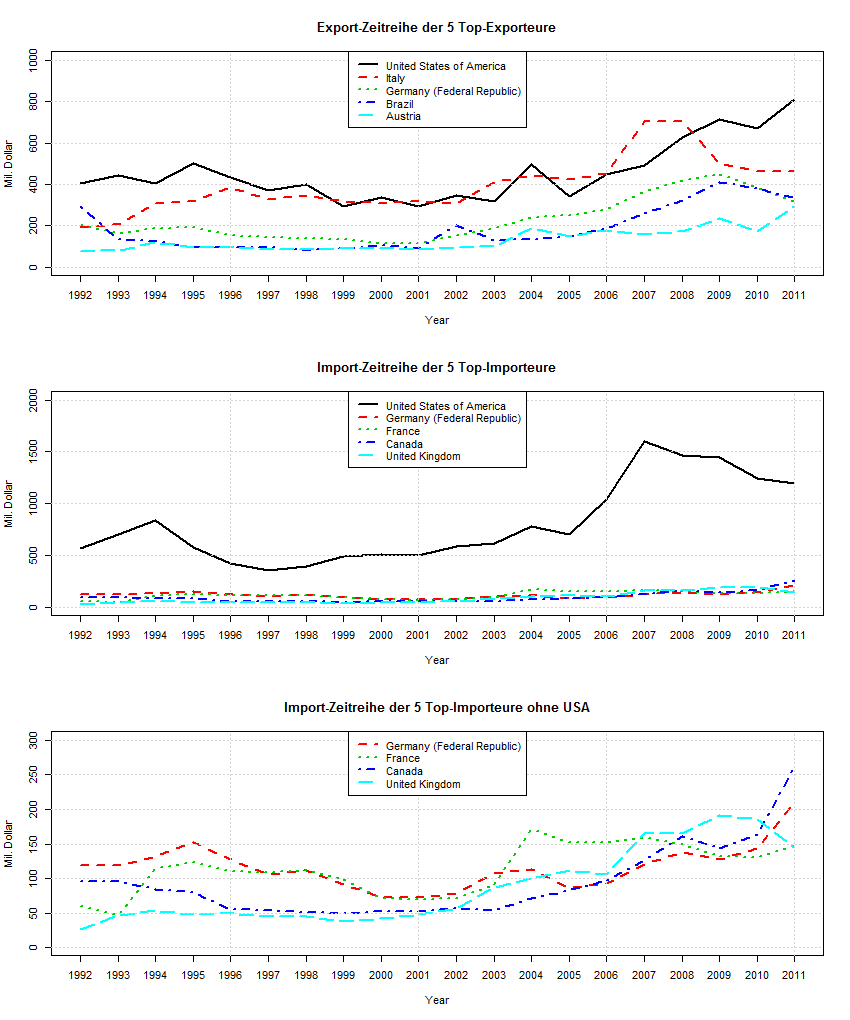
\includegraphics[width=1.00\textwidth]{Grafiken/ts_tops.png}
	\caption{Zeiteihen der Handelswerte der Top-Exporteure/Importeure}
	\label{fig:ts_tops}
\end{figure}
Eine andere Methode, um zentrale Akteure des Netzwerkes zu identifizieren ist sich die Degree-Sequenz der Netzwerkknoten zu betrachten. Welche Knoten (Länder) besitzen sowohl einen hohen In-Degree als auch einen hohen Out-Degree und können somit als zentrale Importeure beziehungsweise Exporteure des Handelsnetzwerkes identifiziert werden?
Abbildung \ref{fig:ts_network} zeigt hierzu das Gesamte Netzwerk in den Jahren 1992, 1996, 2000, 2004, 2008, und 2011. Jeder Punkt stellt ein am Waffenhandel beteiligtes Land dar. Ein Pfeil zwischen den beiden Ländern symbolisiert einen Handel. Länder die aus midestens 30 anderen Ländern Waffen beziehen sind grün, Länder die in midestens 30 andere Länder Waffen liefern sind blau, und Akteure die beide Bedingungen erfüllen sind rot eingefärbt. Man erkennt, dass die Anzahl der "`großen Akteure"' auf dem Kleinwaffenmarkt über die Zeit deutlich zugenommen hat.Die beiden Tabellen \ref{top_1991} und \ref{top_2011}listen diese für das Jahr 1991 und das Jahr 2011 auf:


\begin{figure}[h]
	\centering
		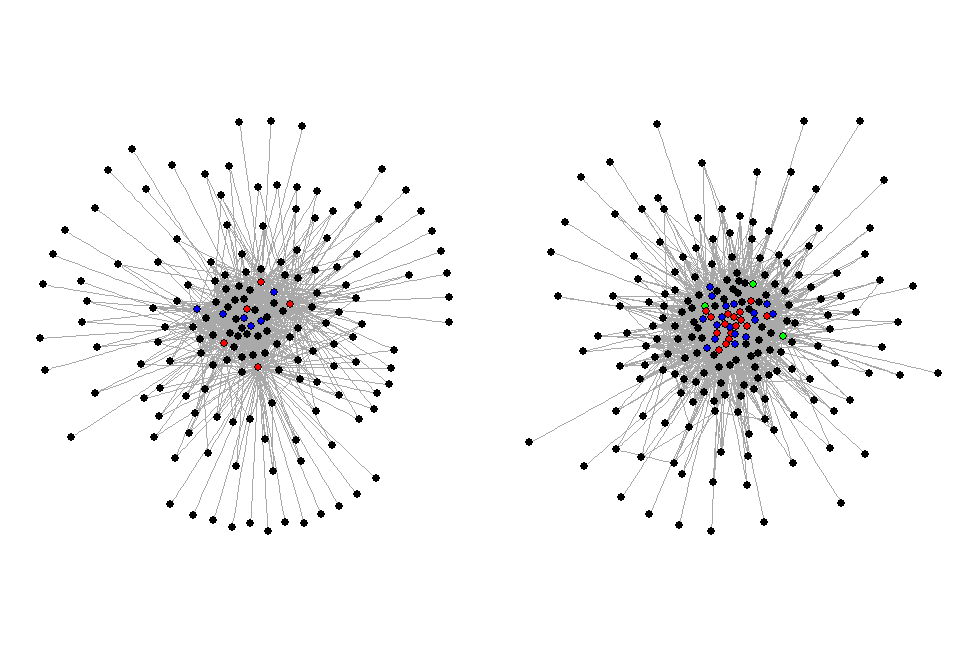
\includegraphics[width=0.90\textwidth]{Grafiken/ts_network.png}
	\caption{Netzwerk im Wandel der Zeit}
	\label{fig:ts_network}
\end{figure}



\begin{table}[h]
\centering
\footnotesize
\begin{tabular}{rlr}
  \hline
 Land 											& In-Degree & Out-Degree\\ 
  \hline
 Switzerland 								& 32				& 76\\ 
 United States of America 	& 43				& 105\\ 
 Germany (Federal Republic) & 47				& 118\\ 
 Spain 											& 36				& 62\\ 
 Sweden 										& 38 				& 33\\ 
 

   \hline
\end{tabular}
\caption{Zentrale Akteure des Netzwerkes 1991} 
\label{top_1991}
	\end{table}
	
	\begin{table}[h]
\centering
\footnotesize
\begin{tabular}{rlr}
  \hline
 Land 						& In-Degree & Out-Degree\\ 
  \hline
 Switzerland 			& 41				& 103\\ 
 United States 		& 63				& 145\\ 
 Finland 					& 34				& 70\\ 
 Italy 						& 39 				& 114\\ 
 France						& 41				& 82\\ 
 Poland						& 32				& 34\\
 Czech Republic		& 37				& 105\\
 Germany					& 50				& 115\\
 United Kongdom		& 44				& 95\\
 Norway						& 32				& 39\\
 Spain  					& 37				& 91\\
 Canada						& 49				& 78\\
 Austria					& 41				& 108\\
 South Africa			& 34				& 32\\
 Belgium					& 31				& 64\\
 Australia				& 39				& 51\\
   \hline
\end{tabular}
\caption{Zentrale Akteure des Netzwerkes 2011} 
\label{top_2011}
	\end{table}



\section{Netzwerkmaßzahlen}

Als zweites erfolgt eine Darstellung grundlegender deskriptiver Netzwerkmaßzahlen, um das Kleinwaffenhandelsnetzwerk zu beschreiben. Die Maßzahlen werden für jedes Jahr berechnet und als Zeitreihe dargestellt, um die zeitliche Entwicklung des Netzwerkes zu visualisieren. 
Abbildung \ref{fig:ts_descriptives} zeigt die zeitliche Entwicklung  von Handelswert, Knotenanzahl, Kantenanzahl und Dichte des Netzwerkes. Betrachtet man zuerst die Zeitreihe der Handelswerte so stellt man fest, dass diese in den Jahren 1992 bis 2001 relativ kostant zwischen 1.5 und 2.5 Milliarden US Dollar verweilt, nach 2001 jedoch bis auf ca 4.5 Milliarden im Jahr 2008 ansteigt und anschließend auf diesem Level konstant bleibt.
Die Zeitreihe der Anzahl der am Waffenhandel beteiligten Nationen steigt recht gleichmäßig zwischen Jahren 1992 und 2011. Lediglich zwischen 1993 und 1994 ist ein außergewöhnlich starker Anstieg von 170 auf 187 zu beobachten. Im Jahr 1997 ist die Anzahl der am Waffenhandel beteiligten Nationen auffallend von 186 auf 176 gesunken. Allerdings stellt sich gleich im Folgejahr wieder die ursprüngliche Anzahl ein. Das Maximum der zeitreihe liegt mit 212 Nationen im Jahr 2008.
Auch die Anzahl der Netzwerkkanten die der Anzahl der vollzogenen Waffentransaktionen zeigt einen regelmäßig steigenden Trend von ca 3000 im Jahr 1992 bis ca 7000 im Jahr 2011. Auch hier erkennen wir einen sprunghaften Anstieg zwischen 1993 und 1994 sowie ein einknicken im Jahr 1996.
Die Dichte des Netzwerkes steigt in den Jahren 1992-1997 rasch von ca 0.04 auf 0.065 und stagniert anschließend auf einem Level zwischen 0.065 und 0.055.
\begin{figure}[h]
	\centering
		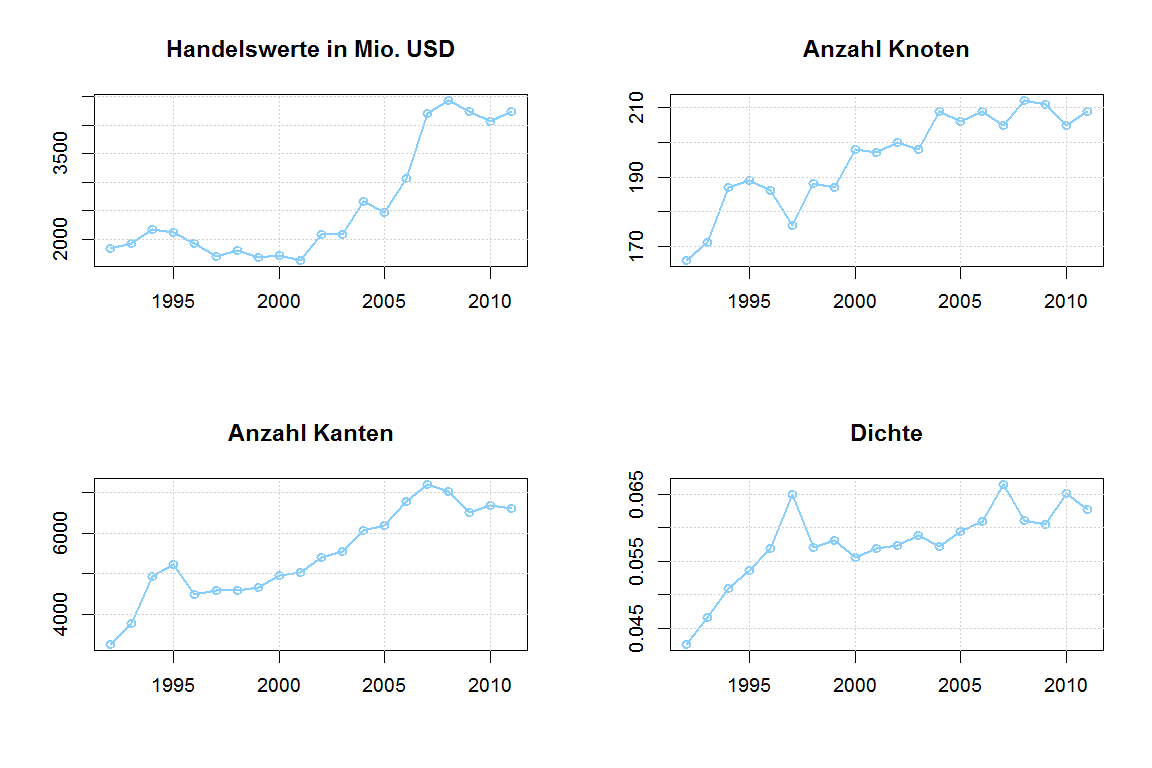
\includegraphics[width=1.00\textwidth]{Grafiken/ts_descriptives.png}
	\caption{Deskripitve Maßzahlen des Kleinwaffenhandelsnetzwerkes 1992-2011}
	\label{fig:ts_descriptives}
\end{figure}
%Die Dichte eines Netzwerkes ist die Anzahl der Kanten des Netzwerkes, geteilt durch die mögliche Anzahl an Kanten des Netzwerkes. Das Kleinwaffenhandelsnetzwerk $G_{NISAT}$ ist ein gerichteter Multigraph mit Schleifen. Da für Multigraphen keine Dichte definiert ist, wird der Graph mit dem Befehl \ttt{simplify(G_Nisat)} auf einen einfachen Graphen reduziert. Die Schleifen im Datensatz werden in der Berechnung der Dichte entfernt. Es ergibt sich der Term $den(G_{NISAT}) = \frac{E_V}{N_H(N_H-1)/2}$ für die Dichte.

\newpage
\section{Visualisierungen}

In diesem Abschnitt wird versucht durch verschiedene Visualisierungen des Netzwerkes einen Überbick über mögliche Strukturen und Zusammenhänge des Kleinwaffenhandels zu erhalten. Da das Netzwerk recht groß ist erscheint es ratsam, die Länder in Gruppen aufzuteilen. Dies geschieht mit Hilfe des R-Pakets \emph{countrycode} \cite{countrycode}. Mit Hilfe der im Datensatz gegeben Correlates of War Country Codes und Zuordnungen der Vereinten Nationen weist dieses Paket jedem Land einen Kontinent bzw ein Jahr zu. In den beiden Grafiken \ref{fig:cont} und \ref{fig:reg} Ist die Größe der Knoten proportional zum jeweiligen Degree (In-Degree + Out-Degree) gewählt. Die Breite der kanten wiederum ist proportional zum monetären Wert der Handelsströme zwsichen zwei Kontinenten beziehungsweise Regionen gwählt. Die Positionierung der Knoten wurde zur besseren Vergleichbarkeit der Jahre untereinander fixiert.

\begin{figure}[!h]
\centering
\animategraphics[scale=0.9, controls]{1}{Grafiken/Cont_Ani/cont}{1}{20}
\caption{Handelsströme zwischen den Kontinenten von 1992-2011}
\label{fig:cont}
\end{figure}

In Abbildung \ref{fig:cont} erkennt man, dass Europa durchgängig mit dem Größten Kreis markeiert ist, also an mehr Handelsaktionen als die anderen Kontinente beteiligt ist. Amerika und Asien folgen auf den nächsten beiden Plätzen. Die Dicke der Kanten und damit der Geldfluss zwischen den Kontinenten variiert stark zwischen den Jahren. Hier ist kein gleichbleibendes Muster zu erkennen.

\begin{figure}[!h]
\centering
\animategraphics[scale=0.9, controls]{1}{Grafiken/Reg_Ani/reg}{1}{20}
\caption{Handelsströme zwischen den Regionen von 1992-2011}
\label{fig:reg}
\end{figure}

In Abbildung \ref{fig:reg} zeigt sich ein ähnliches Bild. Die europäischen Regionen und Nordamerika scheinen die aktivsten Handelspartner zu sein, während immer wieder auch zwischen eher weniger aktiven Regionen große Geldsummen fließen und hier auch wieder kein kostantes Muster zu erkennen ist.  

 

\bibliographystyle{plain}
\bibliography{literatur}


\chapter*{Eidesstattliche Erklärung}

Wir erklären hiermit, dass wir diese Arbeit ohne fremde Hilfe angefertigt und nur die im Literaturverzeichnis aufgeführten Quellen und Hilfsmittel benutzt haben. Diese Arbeit wurde noch nicht zu anderen prüfungsrelevanten Zwecken vorgelegt.\\[1.5cm]

\noindent ................................................
\qquad\qquad\qquad\qquad\qquad
......................................................\\[0.5mm]
\textit{Ort, Datum}
\qquad\qquad\qquad\qquad\qquad\qquad\qquad\qquad\qquad
\textit{Roman Dieterle, Felix Loewe}














\end{document}


